% figures/Borel-separation.tex

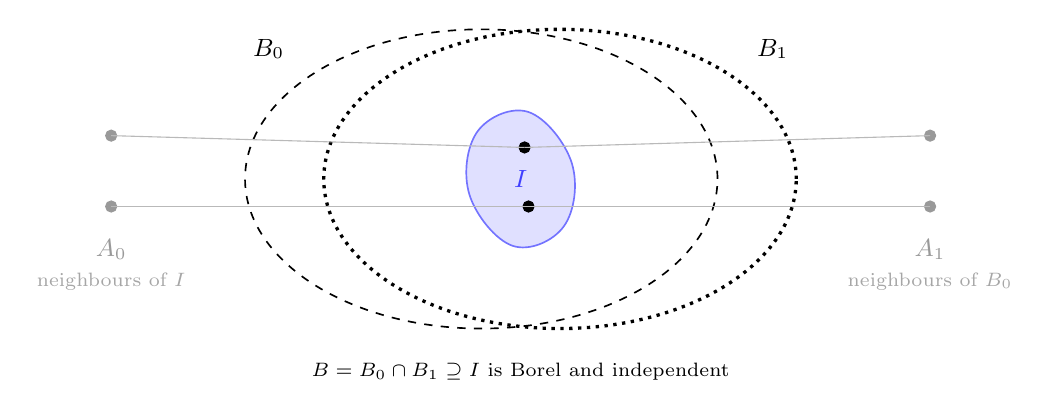
\begin{tikzpicture}[font=\small]

  % B0 -- dashed ellipse, offset left
  \draw[dashed, semithick] (-0.5, 0) ellipse (3.0 and 1.9);
  \node at (-3.2, 1.65) {$B_0$};

  % B1 -- dotted ellipse, offset right
  \draw[dotted, semithick, line width=1.2pt] (0.5, 0) ellipse (3.0 and 1.9);
  \node at (3.2, 1.65) {$B_1$};

  % I -- organic blob sitting in the intersection
  \filldraw[fill=blue!12, draw=blue!55, semithick]
    plot[smooth cycle, tension=0.65] coordinates {
      ( 0.10,  0.85) ( 0.65,  0.20) ( 0.55, -0.60)
      (-0.10, -0.85) (-0.65, -0.20) (-0.55,  0.60)
    };
  \node[blue!75] at (0, 0) {$I$};

  % Two vertices inside I
  \filldraw (0.05,  0.40) circle (2pt) coordinate (v1);
  \filldraw (0.10, -0.35) circle (2pt) coordinate (v2);

  % A0 -- neighbours of I, outside B0  (B0 reaches to x = -3.5)
  \filldraw[gray!80] (-5.2,  0.55) circle (2pt) coordinate (a01);
  \filldraw[gray!80] (-5.2, -0.35) circle (2pt) coordinate (a02);
  \node[gray!80]             at (-5.2, -0.90) {$A_0$};
  \node[gray!70, font=\scriptsize] at (-5.2, -1.30) {neighbours of $I$};

  % A1 -- neighbours of B0, outside B1  (B1 reaches to x = +3.5)
  \filldraw[gray!80] (5.2,  0.55) circle (2pt) coordinate (a11);
  \filldraw[gray!80] (5.2, -0.35) circle (2pt) coordinate (a12);
  \node[gray!80]             at (5.2, -0.90) {$A_1$};
  \node[gray!70, font=\scriptsize] at (5.2, -1.30) {neighbours of $B_0$};

  % Edges from I to A0 (cross the B0 boundary)
  \draw[gray!55, thin] (v1) -- (a01);
  \draw[gray!55, thin] (v2) -- (a02);

  % Edges from I (subset of B0) to A1 (cross the B1 boundary)
  \draw[gray!55, thin] (v1) -- (a11);
  \draw[gray!55, thin] (v2) -- (a12);

  % Caption
  \node[font=\scriptsize] at (0, -2.45)
    {$B = B_0 \cap B_1 \supseteq I$ is Borel and independent};

\end{tikzpicture}